%%
%% For submission/review: [acmsmall,screen,review]
%% For camera-ready:      [acmsmall]
%%
\documentclass[acmsmall,screen,review]{acmart}

%%
%% Author-year citations required by ACM TOMS.
%% Must appear in the preamble, before \begin{document}.
%%
\citestyle{acmauthoryear}

%%
%% Packages approved by ACM TAPS not already included in acmart.
%% Do NOT re-add: amsmath, booktabs, fontenc, inputenc, natbib,
%%                geometry, graphicx, hyperref, microtype, xcolor.
%%
\usepackage{algorithm}
\usepackage{algorithmic}

%%
%% Rights management — replace with values from the ACM rights form.
%%
\setcopyright{acmlicensed}
\copyrightyear{2026}
\acmYear{2026}
\acmDOI{XXXXXXX.XXXXXXX}

\acmJournal{TOMS}
\acmVolume{0}
\acmNumber{0}
\acmArticle{0}
\acmMonth{0}

%%
%% end of preamble
%%
\begin{document}

\title{Algorithm XXXX: pysib, a Python Package for Prediction-Error
       Identification of SISO Polynomial Models}

\author{Diego Eckhard}
\affiliation{%
  \institution{Universidade Federal do Rio Grande do Sul}
  \city{Porto Alegre}
  \country{Brazil}
}
\email{diegoeck@ufrgs.br}
\orcid{0000-0001-8557-0384}

\renewcommand{\shortauthors}{Eckhard}

\begin{abstract}
\texttt{pysib} is an open-source Python package for parameter identification
of discrete-time single-input single-output (SISO) systems described by
linear polynomial input--output models.  It implements the prediction-error
method (PEM) for the ARX, output-error, ARMAX, and Box--Jenkins model
structures; the Steiglitz--McBride iteration and filtered continuation
variants for non-convex prediction-error criteria; and instrumental-variable
and correlation estimators for ARX-structure models under weaker noise
assumptions.  All estimators share a common interface:
they return a parameter vector and a five-polynomial dictionary with entries
\texttt{A}, \texttt{B}, \texttt{C}, \texttt{D}, and \texttt{F}, so models
from different routines can be passed to the same prediction and
simulation functions.  Estimators that reduce to linear algebra are
implemented in Python using NumPy and SciPy.  The PEM estimators for
non-convex criteria follow a deliberately conservative strategy of many small parameter updates
with analytic sensitivity recursions; its many cost, gradient, and
sensitivity evaluations are handled by compiled C extensions with LAPACK
routines for the Gauss--Newton step.  Monte Carlo experiments show that Steiglitz--McBride and
PEM estimates under the output-error structure are centered close to the true
parameters under additive output noise, and that filtered continuation raises
the empirical success rate of the output-error PEM estimator from 60\% to
100\% on a non-convex prediction-error problem.
\end{abstract}

%%
%% CCS concepts — generate the correct codes at https://dl.acm.org/ccs/ccs.cfm
%%
\begin{CCSXML}
<ccs2012>
  <concept>
    <concept_id>10002950.10003705.10003707</concept_id>
    <concept_desc>Mathematics of computing~Mathematical software</concept_desc>
    <concept_significance>500</concept_significance>
  </concept>
  <concept>
    <concept_id>10010147.10010169.10010170</concept_id>
    <concept_desc>Computing methodologies~Simulation and modeling</concept_desc>
    <concept_significance>300</concept_significance>
  </concept>
</ccs2012>
\end{CCSXML}
\ccsdesc[500]{Mathematics of computing~Mathematical software}
\ccsdesc[300]{Computing methodologies~Simulation and modeling}

\keywords{system identification, Python, prediction-error method,
polynomial models, mathematical software}

\maketitle

\section{Introduction}
\label{sec:introduction}

Identifying dynamic models from measured input--output records is a
central problem in control, simulation, and signal processing.
Among the available model classes, discrete-time polynomial
input--output structures---ARX, ARMAX, output-error, and
Box--Jenkins---remain widely used because they are interpretable,
compact, and well supported by the prediction-error
framework~\cite{ljung1999,ljung2010,soderstrom1989}.
Estimating such linear dynamic models from data requires solving a
prediction-error minimization problem.  For ARX structures this criterion is a
convex quadratic least-squares problem, whereas for OE, ARMAX, and
Box--Jenkins structures the same PEM framework generally leads to non-convex
least-squares criteria whose numerical outcome also depends on initialization
and the optimization trajectory.

The MATLAB System Identification Toolbox and the SIB toolbox provide
mature, feature-rich implementations of these classical estimators,
but they are either proprietary or tied to a commercial
platform~\cite{mathworks_sysid,sib_matlab}.
In the open Python ecosystem, the SIPPY package offers a broad
collection of input--output and state-space routines~\cite{sippy},
and the Python Control Systems Library supports control analysis and
design workflows~\cite{pythoncontrol},
while SysIdentPy focuses on nonlinear autoregressive models with
exogenous inputs~\cite{sysidentpy}.
A gap remains for an open-source Python package that is specifically
designed for polynomial input--output model structures, with a specialized
PEM optimization core and a unified model convention that allows
seamless switching between estimators.

\texttt{pysib} fills this gap as a compact software package for SISO
polynomial identification.  It implements classical estimators for ARX,
output-error, ARMAX, and Box--Jenkins structures, including least squares,
Steiglitz--McBride, instrumental variables, correlation error minimization,
PEM, and filtered continuation variants for non-convex PEM criteria.  The
routines are exposed through a small Python API:
each estimator returns a parameter vector and a common five-polynomial model
dictionary, and the same returned model can be passed to shared prediction and
simulation routines.  This convention is intended to make the package usable as
a computational tool rather than as a collection of unrelated functions.
Estimators that reduce to direct linear-algebra problems are written in Python
with NumPy and SciPy; the PEM estimators for non-convex criteria use compiled
C extensions that interface with LAPACK for the Newton step.

The package makes three contributions whose combination distinguishes
it from existing Python tools.
First, it is a focused, open-source, and well-tested toolbox for polynomial
input--output structures, with a documented public API, a layered Python/C
architecture, and a common model representation that lets users switch
between ARX-type, OE, ARMAX, and Box--Jenkins models without changing the
downstream evaluation code.
Second, the PEM estimators for the OE, ARMAX, and BJ structures use a
specialized optimization core that combines analytic sensitivity recursions
with a deliberately conservative search based on many small parameter
updates followed by Gauss--Newton refinement; the large number of cost,
gradient, and sensitivity evaluations demanded by this strategy would be
impractical in interpreted Python loops, so the core is implemented as
compiled C extensions with LAPACK linear solvers.
Third, the package provides open implementations of filtered continuation
methods~\cite{eckhard2013input,eckhard2017cost} for non-convex PEM criteria;
these methods progressively relax data filters to drive the estimate toward
the original PEM criterion, and their effect is evaluated below on a
non-convex OE-structure PEM problem.

The remainder of the article is organized as follows.
Section~\ref{sec:problem-model-classes} defines the prediction-error
problem and the four polynomial model structures.
Section~\ref{sec:algorithms} describes the estimators, the specialized PEM
optimization core, and the filtered
continuation strategy.
Section~\ref{sec:software-organization} describes the public API, the common
model convention, and the software architecture.
Section~\ref{sec:numerical-results} presents Monte Carlo experiments
under noisy data and a study of the filtered continuation strategy
on a non-convex output-error PEM problem.
Section~\ref{sec:conclusion} concludes the article.

\section{Problem and Model Classes}
\label{sec:problem-model-classes}

\subsection{The Identification Problem}
\label{subsec:identification-problem}

Consider a discrete-time single-input single-output (SISO) dynamical system
whose internal structure is unknown.  The system is driven by an input
$u(t) \in \mathbb{R}$ and produces a true output $y_0(t) \in \mathbb{R}$,
where $t$ indexes discrete-time samples.  The relationship is dynamic:
$y_0(t)$ depends on the current and past values of $u$, and possibly on past
values of the output itself.

An identification experiment applies an input signal $u(t)$ to the system for
$N$ time steps.  The output is not measured exactly; what is recorded is
\begin{equation}
    y(t) = y_0(t) + v(t), \qquad t = 1, \ldots, N,
    \label{eq:noisy-output}
\end{equation}
where $v(t)$ is an additive disturbance.  No specific structure is assumed for
$v(t)$ at this stage.

The identification problem is: given the data record
$\mathcal{D}_N = \{u(t),\,y(t)\}_{t=1}^{N}$, determine a parametric model
whose one-step-ahead prediction
$\hat{y}(t \mid t-1;\theta)$---a function of past inputs and outputs, indexed
by a finite-dimensional parameter vector $\theta$---makes the prediction
errors
$\varepsilon(t;\theta) = y(t) - \hat{y}(t \mid t-1;\theta)$ small in a
well-defined sense.  This prediction is distinct from the simulated output,
which is the noise-free response obtained by propagating the plant model from
the input alone.  The choice of model structure and the criterion for
``small'' are the subjects of the following sections.

\subsection{Model Parameterization}
\label{subsec:model-structures}

The data are described by the general polynomial model structure, a
parameterized family of candidate relations between the input, the noise,
and the measured output:
\begin{equation}
    y(t) = \frac{B(q^{-1};\theta)}{A(q^{-1};\theta)\,F(q^{-1};\theta)}\,u(t-n_k)
           + \frac{C(q^{-1};\theta)}{A(q^{-1};\theta)\,D(q^{-1};\theta)}\,e(t),
    \label{eq:general-model}
\end{equation}
where $\theta$ is the vector of free polynomial coefficients to be estimated,
$e(t)$ is a zero-mean white-noise sequence, $q^{-1}$ is the
backward-shift operator ($q^{-1}x(t) = x(t-1)$),
and $n_k \geq 0$ is the input delay in samples.
The polynomials are monic and defined in non-negative powers of $q^{-1}$:
\begin{align*}
    A(q^{-1};\theta) &= 1 + a_1 q^{-1} + \cdots + a_{n_a} q^{-n_a}, \\
    B(q^{-1};\theta) &= b_0 + b_1 q^{-1} + \cdots + b_{n_b-1}q^{-(n_b-1)}, \\
    C(q^{-1};\theta) &= 1 + c_1 q^{-1} + \cdots + c_{n_c} q^{-n_c}, \\
    D(q^{-1};\theta) &= 1 + d_1 q^{-1} + \cdots + d_{n_d} q^{-n_d}, \\
    F(q^{-1};\theta) &= 1 + f_1 q^{-1} + \cdots + f_{n_f} q^{-n_f}.
\end{align*}
In this mathematical parametrization the input delay is carried explicitly by
\(n_k\), and the numerator order \(n_b\) counts only the free coefficients of
\(B\), not the delay.  In the model dictionary returned by an estimator,
however, the delay is stored by prepending \(n_k\) zeros to the \texttt{B}
array.  Thus, the conceptual model keeps \(n_k\) separate from \(B(q^{-1})\),
while the returned software representation encodes the same delay inside
\texttt{m["B"]}.
For a given model structure, $\theta$ contains the coefficients of the
\emph{free} polynomials only (those not fixed to unity).  For example, for
the BJ structure all five polynomials contribute free coefficients, so
$\theta = [b_0,\ldots,b_{n_b-1},\,c_1,\ldots,c_{n_c},\,
           d_1,\ldots,d_{n_d},\,f_1,\ldots,f_{n_f}]^\top$;
for ARX, only $A$ and $B$ are free, giving
$\theta = [a_1,\ldots,a_{n_a},\,b_0,\ldots,b_{n_b-1}]^\top$.
The dimension $n_\theta$ depends on the chosen orders and structure.
The four standard structures are special cases of~\eqref{eq:general-model}
obtained by fixing some polynomials to unity, as listed in
Table~\ref{tab:structures}.
The plant transfer function and noise model are, respectively,
\begin{equation}
    G(q^{-1};\theta) = \frac{B(q^{-1};\theta)}{A(q^{-1};\theta)\,F(q^{-1};\theta)},
    \qquad
    H(q^{-1};\theta) = \frac{C(q^{-1};\theta)}{A(q^{-1};\theta)\,D(q^{-1};\theta)},
    \label{eq:gh}
\end{equation}
so~\eqref{eq:general-model} reads compactly as
$y(t) = G(q^{-1};\theta)\,u(t-n_k) + H(q^{-1};\theta)\,e(t)$.
At the true parameter vector $\theta_0$ this gives
$y_0(t) = G(q^{-1};\theta_0)\,u(t-n_k)$ and
$v(t) = H(q^{-1};\theta_0)\,e(t)$, making precise the
decomposition~\eqref{eq:noisy-output} of
Section~\ref{subsec:identification-problem}.
A key structural distinction
separates the four models: in ARX and ARMAX, the plant denominator and the
noise model share the same polynomial $A$, so the dynamics of the noise
and the plant are coupled; in OE and Box--Jenkins, the plant denominator
$F$ and the noise model $C/D$ are independent, allowing the two components
to be parameterized separately.

\begin{table}[t]
    \caption{Polynomial model structures supported by \texttt{pysib}.
             A free polynomial is estimated from data; a fixed polynomial
             is set to unity.}
    \label{tab:structures}
    \centering
    \footnotesize
    \setlength{\tabcolsep}{4pt}
    \begin{tabular}{lcccccc}
        \toprule
        Structure & $A$ & $B$ & $C$ & $D$ & $F$ & Noise model $H$ \\
        \midrule
        ARX   & free & free & $1$ & $1$ & $1$ & $1/A$ \\
        ARMAX & free & free & free & $1$ & $1$ & $C/A$ \\
        OE    & $1$  & free & $1$ & $1$ & free & $1$ \\
        BJ    & $1$  & free & free & free & free & $C/D$ \\
        \bottomrule
    \end{tabular}
\end{table}

The one-step-ahead predictor associated with the general
structure~\eqref{eq:general-model} is~\cite{ljung1999}
\begin{equation}
    \hat{y}(t \mid t-1;\theta) =
    y(t) + H(q^{-1};\theta)^{-1}
    \bigl[G(q^{-1};\theta)\,u(t-n_k) - y(t)\bigr],
    \label{eq:predictor}
\end{equation}
where $H(q^{-1};\theta)^{-1} = A(q^{-1};\theta)D(q^{-1};\theta)/C(q^{-1};\theta)$.
Substituting the polynomial assignments of Table~\ref{tab:structures}
into~\eqref{eq:predictor} yields the structure-specific predictor.
For the ARX structure,
\begin{equation}
    \hat{y}(t \mid t-1;\theta) =
    \sum_{j=0}^{n_b-1} b_j\,u(t-n_k-j)
    - \sum_{i=1}^{n_a} a_i\,y(t-i),
    \label{eq:arx-predictor}
\end{equation}
which is linear in $\theta$.
For the OE, ARMAX, and Box--Jenkins structures:
\begin{align}
    \hat{y}(t \mid t-1;\theta) &= \frac{B(q^{-1};\theta)}{F(q^{-1};\theta)}\,u(t-n_k),
    && \text{OE}, \label{eq:oe-predictor}\\
    \hat{y}(t \mid t-1;\theta) &= \frac{B(q^{-1};\theta)}{C(q^{-1};\theta)}\,u(t-n_k)
    + \frac{C(q^{-1};\theta)-A(q^{-1};\theta)}{C(q^{-1};\theta)}\,y(t),
    && \text{ARMAX}, \label{eq:armax-predictor}\\
    \hat{y}(t \mid t-1;\theta) &= y(t)
    + \frac{D(q^{-1};\theta)}{C(q^{-1};\theta)}
    \left[\frac{B(q^{-1};\theta)}{F(q^{-1};\theta)}\,u(t-n_k) - y(t)\right],
    && \text{BJ}. \label{eq:bj-predictor}
\end{align}
Thus, for Box--Jenkins models, prediction is evaluated by filtering the
plant-output mismatch through the inverse noise model $D(q^{-1};\theta)/C(q^{-1};\theta)$
and adding the result to the measured output.

\subsection{Parameter Estimation}
\label{subsec:criterion}

The prediction-error method (PEM) estimates $\theta$ by minimizing
the mean squared prediction error~\cite{ljung1999,soderstrom1989}
\begin{equation}
    V(\theta) = \frac{1}{N}\sum_{t=1}^{N} \varepsilon(t;\theta)^2,
    \label{eq:criterion}
\end{equation}
where $\varepsilon(t;\theta) = y(t) - \hat{y}(t \mid t-1;\theta)$ is the
one-step-ahead prediction error.
For the ARX predictor~\eqref{eq:arx-predictor}, writing
$\hat{y}(t \mid t-1;\theta) = \varphi(t)^\top\theta$ with the regression vector
\begin{equation}
  \varphi(t) = \bigl[-y(t-1),\ldots,-y(t-n_a),\,
                      u(t-n_k),\ldots,u(t-n_k-n_b+1)\bigr]^\top,
  \label{eq:regressor}
\end{equation}
and stacking $N$ rows into $\Phi \in \mathbb{R}^{N \times (n_a+n_b)}$ gives
$V(\theta) \propto \|\Phi\theta - y\|^2$,
whose minimum is the ordinary least-squares (OLS) solution
$\hat{\theta} = (\Phi^\top\Phi)^{-1}\Phi^\top y$.

The gradient of~\eqref{eq:criterion} with respect to $\theta$ is
determined by the \emph{sensitivity matrix}
$\Psi(\theta) \in \mathbb{R}^{N \times n_\theta}$, whose $j$-th column collects
\begin{equation}
  \psi_j(t;\theta) = \frac{\partial\hat{y}(t \mid t-1;\theta)}{\partial\theta_j}.
  \label{eq:sensitivity}
\end{equation}
Since $\varepsilon(t;\theta) = y(t) - \hat{y}(t \mid t-1;\theta)$, the chain rule gives
\begin{equation}
  \frac{\partial V}{\partial\theta} = -\frac{2}{N}\,\Psi(\theta)^\top\varepsilon(\theta),
  \label{eq:gradient-v}
\end{equation}
where $\varepsilon(\theta) = [\varepsilon(1;\theta),\ldots,\varepsilon(N;\theta)]^\top$.
For the ARX structure, $\psi_j(t;\theta) = \varphi_j(t)$ (the $j$-th entry of
the regression vector~\eqref{eq:regressor}), and~\eqref{eq:gradient-v} vanishes
exactly at the OLS solution.  For the OE, ARMAX, and Box--Jenkins structures, $\psi_j$
requires filtering through $1/F(q^{-1})$ or $1/C(q^{-1})$---polynomials
that depend on $\theta$ itself---making $\Psi$ a nonlinear function of
$\theta$ and~\eqref{eq:criterion} non-convex in general; the existence
of multiple local minima for these linear model structures is well
documented~\cite{astrom1974,soderstrom1982,eckhard2011global,eckhard2012pem}.  The
Gauss--Newton approximation to the Hessian,
\begin{equation}
  \frac{\partial^2 V}{\partial\theta^2} \approx \frac{2}{N}\,\Psi^\top\Psi,
  \label{eq:gn-hessian-fw}
\end{equation}
retains only the outer-product term (dropping second-order sensitivity
terms that vanish near the minimum).  It is symmetric positive semidefinite
by construction; when the sensitivity matrix $\Psi$ has full column rank
the Gram matrix $\Psi^\top\Psi$ becomes positive definite and the
Gauss--Newton direction is well defined and points downhill.
Under standard regularity conditions on the input and noise,
global minimizers of the PEM criterion are consistent when the
true system belongs to the model class~\cite{ljung1978,ljung1999};
the implemented PEM routines for non-convex criteria seek such minima through
local optimization, so the numerical outcome also depends on
initialization and the optimizer.

Several estimators in \texttt{pysib} avoid direct local optimization of a
non-convex PEM criterion.  They differ in their target model structure: SM
targets the OE plant structure \(G = B/F\), whereas IV and correlation target
ARX-structure models.

\paragraph{Steiglitz--McBride (SM)}
The SM method~\cite{steiglitz1965} replaces the non-convex OE-structure PEM
problem with a sequence of ARX least-squares problems solved on filtered
data.  The ARX step is computational, not the model structure ultimately
reported: the returned estimate is an OE-structure plant model \(G=B/F\),
and no disturbance model \(H\) is identified.  The iteration, its
fixed-point properties, and the implementation choices are described in
Section~\ref{subsubsec:sm}.

\paragraph{Instrumental Variables (IV)}
The IV method estimates an ARX model consistently even when the noise
is not of the form $1/A(q^{-1};\theta)\,e(t)$, at the cost of requiring two
independent experiments driven by the same input $u(t)$.  Let
$y_i(t) = y_0(t) + e_i(t)$, $i = 1,2$, denote the noisy outputs, where
$y_0(t)$ is the true plant output and $e_1(t)$, $e_2(t)$ are independent
noise sequences.  Define the regression matrix
$\Phi_1 \in \mathbb{R}^{N \times (n_a+n_b)}$ with rows
\[
  \varphi_1(t)^\top = \bigl[-y_1(t-1),\ldots,-y_1(t-n_a),\,
                             u(t-n_k),\ldots,u(t-n_k-n_b+1)\bigr],
\]
and the instrument matrix $Z \in \mathbb{R}^{N \times (n_a+n_b)}$ with rows
\[
  \zeta(t)^\top = \bigl[-y_2(t-1),\ldots,-y_2(t-n_a),\,
                         u(t-n_k),\ldots,u(t-n_k-n_b+1)\bigr],
\]
where the lagged $y_1$ entries of $\varphi_1$ are replaced by the
corresponding lagged $y_2$ entries.  The IV estimate is
\begin{equation}
    \hat{\theta} = (Z^\top \Phi_1)^{-1} Z^\top y_1.
    \label{eq:iv}
\end{equation}
Because $Z$ shares the input-driven part of $\Phi_1$ but $Z^\top e_1 \to 0$
as $N \to \infty$ (since $e_2$ and $e_1$ are independent),
$\hat{\theta}$ is consistent~\cite{soderstrom1989}.

\paragraph{Correlation method.}
The correlation method finds $\theta$ by requiring the prediction error
$\varepsilon(t;\theta)$ to be uncorrelated with an instrument $z(t)$ at
$M$ lags:
\begin{equation}
    \frac{1}{N}\sum_t z(t-\tau)\,\varepsilon(t;\theta) = 0,
    \qquad \tau = 0,1,\ldots,M-1.
    \label{eq:correlation}
\end{equation}
Since $\varepsilon(t;\theta)$ is linear in $\theta$ for the ARX structure,
\eqref{eq:correlation} constitutes a system of $M$ linear equations.
For $M = n_a + n_b$ the system is exactly determined; for $M > n_a + n_b$
it is overdetermined and solved by least squares, which minimizes the sum
of squared cross-correlations.

These estimators can be applied directly when their respective assumptions are
appropriate.  In addition, the ARX least-squares routine provides the initial
parameter vector for every PEM estimator whose criterion is optimized
iteratively in \texttt{pysib}: each such routine is warm-started from an ARX
solution, so the optimizer begins from a meaningful point rather than an
arbitrary initial guess.

\section{Algorithms}
\label{sec:algorithms}

\subsection{Linear-Algebra-Based Estimators}
\label{subsec:linear-estimators}

\subsubsection{ARX}
\label{subsubsec:arx}

The ARX estimator is the fundamental least-squares routine in the package and
the warm-start for every iterative PEM routine.
The ARX predictor~\eqref{eq:arx-predictor} is linear in $\theta$:
$\hat{y}(t \mid t-1;\theta) = \varphi(t)^\top\theta$,
where $\varphi(t)$ is the regression vector~\eqref{eq:regressor}.
Stacking $N$ rows into the regression matrix
$\Phi \in \mathbb{R}^{N \times n_\theta}$ and the outputs into
$y = [y(1),\ldots,y(N)]^\top \in \mathbb{R}^N$,
the PEM criterion~\eqref{eq:criterion} reduces to
\[
    V(\theta) = \frac{1}{N}\,\|\Phi\theta - y\|^2,
\]
which is a convex quadratic function of $\theta$ (the Hessian
$\frac{2}{N}\Phi^\top\Phi$ is positive semidefinite).
Differentiating and setting $\partial V/\partial\theta = 0$ yields the
\emph{normal equations}
\[
    \Phi^\top\Phi\,\hat\theta = \Phi^\top y.
\]
The solution is unique if and only if $\Phi$ has full column rank, i.e.,
$\Phi^\top\Phi$ is invertible, in which case
$\hat\theta = (\Phi^\top\Phi)^{-1}\Phi^\top y$ is the unique global
minimum of $V(\theta)$.  Full column rank is obtained in open-loop identification when the input
$u(t)$ is \emph{persistently exciting} of order $n_\theta$: informally,
the input must contain enough distinct frequency components to excite all
modes of the regression matrix~\cite{ljung1999}.  When this condition
fails (e.g., a constant or insufficiently rich input), $\Phi$ is
rank-deficient and $V(\theta)$ has infinitely many minimizers forming an
affine subspace.

Computing $(\Phi^\top\Phi)^{-1}$ directly is numerically inadvisable
even in the full-rank case: the condition number satisfies
$\kappa(\Phi^\top\Phi) = \kappa(\Phi)^2$, so any ill-conditioning in
$\Phi$ is squared, amplifying rounding errors.  \texttt{pysib} instead
calls \texttt{numpy.linalg.lstsq}, which invokes the LAPACK driver
\texttt{dgelsd}.  This routine solves the least-squares problem via the
divide-and-conquer SVD of $\Phi$ directly, avoiding the normal equations
entirely.  When $\Phi$ is rank-deficient, \texttt{dgelsd} returns the
minimum-norm solution among all minimizers of $V(\theta)$.

\subsubsection{Steiglitz--McBride}
\label{subsubsec:sm}

The OE-structure predictor
$\hat{y}(t \mid t-1;\theta) = B(q^{-1};\theta)/F(q^{-1};\theta)\,u(t-n_k)$
is nonlinear in the $F$ coefficients, making the PEM criterion
$V(\theta)$ non-convex even though the model is linear in the input and noise.
The SM method approximates the OE-structure PEM solution by replacing the
single non-convex problem with a sequence of auxiliary ARX least-squares
problems.

At each iteration $k$, the current denominator estimate
$\hat{F}^{(k)}(q^{-1};\theta)$ is used to prefilter both signals:
\[
  u_f(t) = \frac{u(t)}{\hat{F}^{(k)}(q^{-1};\theta)}, \qquad
  y_f(t) = \frac{y(t)}{\hat{F}^{(k)}(q^{-1};\theta)}.
\]
An auxiliary ARX least-squares problem of orders $(n_f, n_b)$ is then solved
on the filtered pair $(u_f, y_f)$ using the procedure of
Section~\ref{subsubsec:arx}, and the new denominator estimate
$\hat{F}^{(k+1)}$ is taken from the feedback polynomial of that auxiliary
solution.
When the additive disturbance $v(t)$ is white noise, a fixed point
$\hat{F}^{(k+1)} = \hat{F}^{(k)}$ of this iteration satisfies the
optimality conditions of the OE-structure PEM criterion; for colored
disturbances, however, the fixed points are in general not stationary
points of $V(\theta)$ and the SM estimate is
biased~\cite{stoica1981,ljung1999}.  Convergence to the global minimum is
not guaranteed even in the white-noise case, and the result depends on the
initialization.  \texttt{pysib} initializes $\hat{F}^{(0)}$
from a plain ARX solution on the unfiltered data.  The implementation uses the
fixed iteration count \(K=100\): each iteration filters \(u\) and \(y\) by the
current denominator estimate, calls the ARX routine on the filtered pair, and
updates the OE denominator from the feedback polynomial of the auxiliary ARX
result.  The final SM model contains only the OE plant polynomials \(B\) and
\(F\); it does not estimate a separate noise model \(H\).

\subsubsection{Instrumental Variables}
\label{subsubsec:iv}

The IV estimator solves the linear system
$(Z^\top\Phi_1)\,\hat\theta = Z^\top y_1$,
where $\Phi_1$ and $Z$ are the regression and instrument matrices
defined in Section~\ref{subsec:criterion}.
The system is solved by least squares via
\texttt{numpy.linalg.lstsq}.
Consistency requires the noise sequences of the two experiments to be
mutually uncorrelated and uncorrelated with the input
(Section~\ref{subsec:criterion}).
In \texttt{pysib}, the IV routine accepts a single pair
$(u, y_1)$ and a second output record $y_2$; when the two outputs
are identical, the method reduces to ordinary least-squares ARX.

\subsubsection{Correlation}
\label{subsubsec:correlation}

The correlation estimator assembles the $M \times (n_a+n_b)$ matrix
of cross-correlations between the instrument $z(t)$ and the lagged
signals that appear in the ARX predictor, together with the
corresponding right-hand side.
The default instrument is $z = u$, which is valid in open-loop
experiments where the input is uncorrelated with the noise.
The linear system~\eqref{eq:correlation} is solved via
\texttt{numpy.linalg.lstsq}, which in the overdetermined case
$M > n_a + n_b$ yields the solution described in
Section~\ref{subsec:criterion}.
The implementation follows the same pattern as ARX: the regressor
matrix is assembled once and the result returned without iteration.

\subsection{PEM Estimators for Non-Convex Criteria and Optimization Core}
\label{subsec:nonlinear-optimization-core}

The OE, ARMAX, and Box--Jenkins routines estimate linear polynomial model
structures by minimizing the PEM criterion $V(\theta)$ using the
gradient~\eqref{eq:gradient-v} and the Gauss--Newton
Hessian~\eqref{eq:gn-hessian-fw}.  Since the filters in these structures
depend on the parameters, the resulting criteria are generally non-convex.
For this reason, \texttt{pysib} uses a specialized optimization core rather
than treating these estimation problems as generic black-box minimizations.
Local convergence of maximum-likelihood and prediction-error iterations for
ARMAX-type models is known to depend on problem-specific
conditions~\cite{goodwin2003}, so the implementation emphasizes reproducible
safeguards rather than a general convergence guarantee.
The core combines structure-specific sensitivity recursions with a
conservative search strategy based on many small parameter updates, followed
by Gauss--Newton refinement.  This design increases the number of error,
gradient, and sensitivity evaluations, and the performance-critical routines
are therefore implemented as compiled C extensions; the Newton system is
solved through LAPACK.  Each estimator is initialized from an ARX solution;
the free coefficients of the noise-model polynomials $C$ and $D$ are
initialized to zero, so that initially $C = D = 1$.

\paragraph{Structure-specific sensitivities.}
These PEM estimators use analytic, structure-specific sensitivity
recursions rather than numerical differentiation.  Separate C modules are
used for OE, ARMAX, and Box--Jenkins because the free polynomials and the
filters appearing in the sensitivity equations differ across structures.
For the OE predictor
$\hat{y}(t \mid t-1;\theta) = B(q^{-1})/F(q^{-1})\,u(t-n_k)$, for example,
the sensitivities~\eqref{eq:sensitivity} are
\begin{align}
  \psi_{b_j}(t) &= \frac{q^{-j}\,u(t-n_k)}{F(q^{-1})},
                 \label{eq:sens-b} \\
  \psi_{f_j}(t) &= -\frac{q^{-j}\,\hat{y}(t \mid t-1;\theta)}{F(q^{-1})}.
                 \label{eq:sens-f}
\end{align}
For ARMAX the denominator filter is $1/C(q^{-1})$; for Box--Jenkins both
$1/F(q^{-1})$ and $1/C(q^{-1})$ appear, together with the corresponding
noise-model polynomials.  Thus each C module implements the sensitivity
recursions for its own polynomial structure.

\paragraph{Reuse of filtered sensitivity sequences.}
The C implementation also exploits the shift structure of polynomial
models.  Many sensitivity columns differ only by a delay.  In these cases,
the code first computes a filtered base sequence and then forms the
corresponding columns by time shifts, instead of applying the same IIR
filter separately for every coefficient.  In the OE case, a single pass
through $1/F(q^{-1})$ applied to the delayed input provides the base
sequence for all numerator sensitivities, while a single pass applied to
$-\hat{y}$ provides the base sequence for the denominator sensitivities;
the columns associated with $b_j$ and $f_j$ are obtained by indexing these
sequences with the appropriate lag.  The same principle is used in the
ARMAX and Box--Jenkins modules with their respective filters.  This reuse is
important because the optimizer evaluates the cost, gradient, and
Gauss--Newton matrices many times along a single identification run.

\paragraph{Selective cost, gradient, and Hessian evaluation.}
The optimization core distinguishes between three levels of computation.
When only a candidate parameter vector must be accepted or rejected, it
evaluates the cost $V(\theta)$ without forming sensitivities.  During the
initial descent phase, it evaluates the cost and gradient but does not build
the Gauss--Newton matrix.  During the Newton phase, it evaluates the cost,
gradient, and the matrix $\Psi^\top\Psi$ needed in
\eqref{eq:newton-system}.  This separation avoids unnecessary gradient or
Hessian assembly during the many small trial steps used by the optimizer.
For scalar cost comparisons the C core internally uses the
root-mean-square prediction error \smash{$\sqrt{V(\theta)}$}, which
does not change minimizers or accept/reject ordering because it is
strictly increasing in~$V$; the gradient and Gauss--Newton quantities
retain the standard least-squares scaling and are unaffected by a
constant factor in the cost.

\begin{algorithm}
\caption{PEM optimization core for non-convex criteria}
\label{alg:nonlinear-pem-core}
\begin{algorithmic}[1]
\REQUIRE initial parameter vector \(\theta\), cost \(J\), gradient \(g\), sensitivity matrix \(\Psi\)
\STATE initialize \(d\) as undefined, \(\alpha \leftarrow 10^{-5}\)
\FOR{up to \(10^4\) descent updates}
  \STATE compute \(J(\theta)\) and \(g(\theta)\)
  \IF{\(d\) is undefined}
    \STATE \(d \leftarrow g(\theta)\)
  \ELSE
    \STATE \(d \leftarrow (4d + g(\theta))/5\)
  \ENDIF
  \STATE \(\theta_c \leftarrow \theta - \alpha d/\|d\|\)
  \IF{\(J(\theta_c) \leq J(\theta)\)}
    \STATE \(\theta \leftarrow \theta_c\), \(\alpha \leftarrow 1.01\alpha\)
  \ELSE
    \STATE \(\alpha \leftarrow 0.99\alpha\)
  \ENDIF
  \IF{\(\alpha < 10^{-7}\)}
    \STATE stop descent phase
  \ENDIF
\ENDFOR
\FOR{\(k = 1,\ldots,1000\)}
  \STATE compute \(g(\theta)\), \(\Psi(\theta)\), and \(J(\theta)\)
  \STATE solve \((\Psi^\top\Psi)\delta = -\Psi^\top\varepsilon\)
  \STATE \(\theta_c \leftarrow \theta - (k/1000)\delta\)
  \STATE bisect \(\theta_c\) toward \(\theta\) until \(J(\theta_c) \leq J(\theta)\) or the trial budget is exhausted
  \IF{\(J(\theta_c) \leq J(\theta)\)}
    \STATE \(\theta \leftarrow \theta_c\)
  \ENDIF
\ENDFOR
\STATE \RETURN \(\theta\)
\end{algorithmic}
\end{algorithm}

\paragraph{Two-phase optimizer.}
\emph{Phase~1} is a conservative smoothed steepest-descent loop intended to
stabilize the trajectory from the ARX warm start before local Newton
refinement.  At each of up to $10^4$ gradient evaluations, the
gradient $g = \partial V/\partial\theta$~\eqref{eq:gradient-v} is accumulated
by an exponential moving average, $d \leftarrow (4d + g)/5$, which damps
iteration-to-iteration changes in the descent direction.  The direction is
normalized to unit length, separating the direction of motion from the step
size, and the parameter vector is updated by
$\theta \leftarrow \theta - \alpha\,d/\|d\|$.  The step size $\alpha$ adapts
slowly and multiplicatively: $\alpha \leftarrow 1.01\,\alpha$ when the cost
does not increase and $\alpha \leftarrow 0.99\,\alpha$ on an increase, starting
from $\alpha = 10^{-5}$.  The phase terminates early when
$\alpha < 10^{-7}$; in the implementation this test is applied once per
block of $100$ updates.

\emph{Phase~2} performs local Gauss--Newton refinement using the structured
sensitivities computed by the C module.  At each of $1000$ iterations the
Newton direction $\delta$ is obtained by solving
\begin{equation}
  (\Psi^\top\Psi)\,\delta = -\Psi^\top\varepsilon
  \label{eq:newton-system}
\end{equation}
via the LAPACK routine \texttt{dposv}, which solves the Gauss--Newton
normal system by Cholesky factorization under the assumption of positive
definiteness.  The candidate
$\theta \leftarrow \theta - \alpha_k\,\delta$ uses a growing step
$\alpha_k = k/1000$, ranging from $0.001$ at the first iteration to
approximately $1$ at the last, so full Newton steps are approached gradually.
If the candidate increases the cost or is non-finite, a bisection
safeguard is applied up to ten times:
$\theta^{\mathrm{new}} \leftarrow (\theta^{\mathrm{new}} + \theta)/2$.
Phase~2 always performs the full $1000$ iterations, with no
early-termination test: the cost of the refinement phase is fixed by
design, consistent with the conservative strategy of the core.

\subsection{Filtered Continuation Estimators}
\label{subsec:filtered-continuation-estimators}

Non-convex prediction-error criteria may have multiple local minima, and
even a conservative optimizer may converge to a nonglobal stationary point.
The filtered estimators in \texttt{pysib} provide open implementations of
the continuation and cost-function-shaping strategies developed for this
setting~\cite{eckhard2013input,eckhard2017cost}.  At each continuation
stage, filtering the input--output data modifies the shape of the cost
function; progressively relaxing the filter then drives the estimate toward
the original unfiltered criterion.  Filtered variants are provided for the
OE, ARMAX, and Box--Jenkins structures; in each case the final stage
runs the corresponding unfiltered PEM estimator on the original criterion.

\paragraph{Stage sequence and warm-starting.}
The procedure runs nine filtered optimization stages followed by one
final stage on the unfiltered data.  Each stage calls the same PEM
optimization core used by the corresponding unfiltered estimator, but on a
filtered version of the input--output record.  The solution returned by one
stage is used as the initial condition for the next stage, so the
continuation path begins from a strongly shaped criterion and ends at the
original PEM problem.  The total computational cost is approximately ten
times that of the corresponding unfiltered estimator.

\begin{algorithm}
\caption{Filtered continuation wrapper}
\label{alg:filtered-continuation}
\begin{algorithmic}[1]
\REQUIRE data \(u,y\), model orders, PEM estimator \(E\), filter poles \(a_1,\ldots,a_9\)
\STATE \(u_f,y_f \leftarrow\) filter \(u,y\) with pole \(a_1\)
\STATE \(\theta \leftarrow\) ARX-based estimate from \(u_f,y_f\), converted to the parameter order of \(E\)
\FOR{\(i = 1,\ldots,9\)}
  \STATE \(u_f,y_f \leftarrow\) filter \(u,y\) with pole \(a_i\)
  \STATE \(\theta \leftarrow E(u_f,y_f,\mathrm{orders};\theta)\)
\ENDFOR
\STATE \(\theta \leftarrow E(u,y,\mathrm{orders};\theta)\)
\STATE construct the common model dictionary \(m\)
\STATE \RETURN \((\theta,m)\)
\end{algorithmic}
\end{algorithm}

\paragraph{Filter schedule.}
For the OE, ARMAX, and Box--Jenkins structures, each stage uses a first-order IIR filter
$(1-a_i)/(1 - a_i q^{-1})$ with unit DC gain, whose pole is
$a_i = 0.05^{1/\tau_i}$ with $\tau_i = 4(10 - i)$ for stages
$i = 1,\ldots,9$.  The pole decreases from $a_1 \approx 0.920$
(aggressive low-pass, stage~1) to $a_9 \approx 0.473$ (mild
low-pass, stage~9), progressively restoring high-frequency content.
The final stage is the original unfiltered
estimator applied to the same PEM criterion; the only difference
between the standard and filtered routines is the initial
condition---the standard routine starts from an ARX estimate,
while the filtered routine starts from the solution of the
previous filtered stage.

The numerical experiments in
Section~\ref{sec:numerical-results} focus on the OE structure because
the theoretical analysis of cost-function shaping was developed
specifically for the output-error
case~\cite{eckhard2013input,eckhard2017cost}.
The same continuation strategy is implemented for ARMAX and
Box--Jenkins in \texttt{pysib} under the expectation that the mechanism
of progressively relaxing data filters should also improve convergence
in those structures, although formal guarantees have not been
established for them.

\section{Software Interface and Organization}
\label{sec:software-organization}

\texttt{pysib} is designed around a small public API rather than around
separate estimator-specific model objects.  The user supplies one-dimensional
input and output arrays and the requested polynomial orders.  Every estimation
routine returns a pair $(\hat\theta, m)$: the vector $\hat\theta$ contains the
free estimated parameters in the order used by the corresponding algorithm,
whereas $m$ is the model representation used by the rest of the package.  This
separation lets users inspect the numerical parameter vector when needed, while
all prediction, simulation, and comparison routines operate on a common
polynomial model.

The model $m$ is a Python dictionary with keys \texttt{A}, \texttt{B},
\texttt{C}, \texttt{D}, and \texttt{F}.  Each entry is a one-dimensional array
containing the coefficients of the corresponding polynomial in
Section~\ref{subsec:model-structures}; polynomials fixed by a model structure
are stored as the scalar polynomial \texttt{[1]}.  The same convention is used
by the direct linear-algebra estimators, the iterative PEM estimators, and the
filtered continuation variants.  As a result, downstream code does not depend on which
routine produced the model.

Table~\ref{tab:public-api} summarizes the public routines.  Each estimation
routine takes the data arrays, the requested polynomial orders, and the
delay \(n_k\), consistently with Section~\ref{subsec:model-structures}; the
order \(n_b\) counts the free numerator coefficients, not the leading zeros
used internally to store the delay in the returned \texttt{B} polynomial.
The exact signatures of all routines are documented in the user manual.

\begin{table}[t]
    \caption{Public routines in \texttt{pysib}.}
    \label{tab:public-api}
    \centering
    \footnotesize
    \setlength{\tabcolsep}{4pt}
    \begin{tabular}{p{0.28\columnwidth}p{0.55\columnwidth}}
        \toprule
        Routine & Estimator or role \\
        \midrule
        \texttt{arx} & Least squares for the ARX structure \\
        \texttt{sm} & Steiglitz--McBride iteration for the OE structure \\
        \texttt{iv} & Instrumental variables for the ARX structure \\
        \texttt{correlation} & Correlation estimator for the ARX structure \\
        \texttt{oe} & PEM for the OE structure \\
        \texttt{armax} & PEM for the ARMAX structure \\
        \texttt{bj} & PEM for the Box--Jenkins structure \\
        \texttt{oe\_filtered} & Filtered PEM for the OE structure \\
        \texttt{armax\_filtered} & Filtered PEM for the ARMAX structure \\
        \texttt{bj\_filtered} & Filtered PEM for the BJ structure \\
        \texttt{predict} & One-step-ahead prediction \\
        \texttt{simulate} & Noise-free plant simulation \\
        \bottomrule
    \end{tabular}
\end{table}

The routines also have distinct modeling roles.  The \texttt{arx} routine is
the basic least-squares estimator for the ARX structure and the default warm
start for the iterative PEM routines.  \texttt{sm} provides a classical
iterative approximation to PEM estimation of the OE plant structure \(G=B/F\);
internally it solves ARX least-squares subproblems, but its returned model uses
the OE structure and does not include a fitted noise model.  \texttt{iv} and
\texttt{correlation} are alternative estimators for ARX-structure models in
settings where the ordinary least-squares assumptions are unsuitable.
The \texttt{oe}, \texttt{armax}, and \texttt{bj} routines call the PEM
optimizer for non-convex criteria described in
Section~\ref{subsec:nonlinear-optimization-core}.
The three filtered routines expose the continuation strategy of
Section~\ref{subsec:filtered-continuation-estimators} through the same
interface and return the same model dictionary.

A typical workflow estimates a model with one routine and evaluates it with
the shared routines: a call to an estimator such as \texttt{oe} returns the
pair $(\hat\theta, m)$, and the same dictionary $m$ is then passed to
\texttt{predict} and \texttt{simulate}, while its polynomial entries can be
inspected directly.  \texttt{predict} computes the one-step-ahead predictor
\(\hat{y}(t \mid t-1;\hat\theta)\), using the full plant and disturbance model
represented by \(G\) and \(H\).  In contrast, \texttt{simulate} computes the
noise-free simulated output \(\hat{y}_s(t;\hat\theta)\) and uses only the
deterministic transfer function \(G\).  This distinction is important in the
numerical experiments below, where the relative simulation error is intended to
measure the identified plant dynamics rather than the one-step prediction fit.
Complete, runnable examples of every public routine are given in the user
manual.

The package separates Python-level orchestration from performance-critical
compiled routines.  The ARX, IV, and correlation estimators, together with the
auxiliary ARX least-squares subproblems used by SM, are implemented in Python
using NumPy and SciPy.  The PEM optimizers for non-convex criteria
are compiled as three separate C extension modules
(\texttt{sib\_oe\_module.c}, \texttt{sib\_armax\_module.c},
\texttt{sib\_bj\_module.c}), each providing the structure-specific
sensitivity formulas and sharing the common two-phase optimizer from
\texttt{sib\_optimize.c}.  The Newton step in Phase~2 links against
LAPACK (\texttt{dposv}) without requiring an external system identification
framework.  The filtered variants are Python wrappers that sequence the
filter stages and delegate each optimization to the corresponding C module.

This article describes the algorithms, interface, and high-level organization
of the software.  Installation instructions, dependency versions, complete API
documentation, callable-procedure examples, and expected driver outputs are
provided in the accompanying user manual, as required for the CALGO software
component.  Future updated versions of the software package will be made
available via the source repository~\cite{pysib_repo}.

Table~\ref{tab:architecture} summarizes the main implementation components.

\begin{table}[t]
    \caption{Main software components of \texttt{pysib}.}
    \label{tab:architecture}
    \centering
    \footnotesize
    \setlength{\tabcolsep}{3pt}
    \begin{tabular}{p{0.30\columnwidth}p{0.30\columnwidth}p{0.27\columnwidth}}
        \toprule
        Component & Implementation & Role \\
        \midrule
        ARX, IV, Correlation & Python, NumPy, SciPy & ARX-structure estimators \\
        SM & Python, NumPy, SciPy & OE-structure iteration via ARX subproblems \\
        OE, ARMAX, BJ & C extension, LAPACK & PEM for non-convex criteria \\
        Filtered variants & Python over C optimizer & Continuation strategy \\
        Prediction and simulation & SciPy \texttt{lfilter} & Model evaluation \\
        \bottomrule
    \end{tabular}
\end{table}

\begin{table}[t]
    \caption{Software artifact summary.}
    \label{tab:artifact}
    \centering
    \footnotesize
    \setlength{\tabcolsep}{4pt}
    \begin{tabular}{p{0.28\columnwidth}p{0.60\columnwidth}}
        \toprule
        Item & Description \\
        \midrule
        Language & Python package with compiled C extensions \\
        Numerical libraries & NumPy, SciPy, and LAPACK \\
        License & MIT \\
        Documentation & User manual included with the CALGO artifact \\
        Tests & Unit tests covering all public estimation routines \\
        Experiments & Reproducible drivers for the numerical results in this article \\
        Artifact contents & Source code, user manual, tests, experiment drivers, and expected outputs \\
        \bottomrule
    \end{tabular}
\end{table}

\section{Numerical Results}
\label{sec:numerical-results}

The accompanying software artifact includes deterministic unit tests for
noise-free exact recovery and for the polynomial convention of
Section~\ref{sec:problem-model-classes}.  These tests cover all public
estimators---ARX, SM, IV, correlation, OE, ARMAX,~BJ, and the filtered
variants---on low-order systems with known parameters, and they exercise the
common return convention used by the \texttt{predict} and \texttt{simulate}
routines.
They are part of the software validation and are not presented as
scientific results.  The numerical experiments reported here are reproducible
drivers included with the artifact.  They illustrate two end-to-end uses of
the package: estimating models under noisy data and evaluating the effect of
filtered continuation in a non-convex PEM problem.  The purpose is
to validate representative software workflows and numerical behavior, not to
provide a general benchmark of all available system-identification packages.

\subsection{Robustness under Noisy Data}
\label{subsec:robustness-noisy-data}

The first experiment evaluates the SM and OE estimators under additive
white output noise.
The driver follows the same workflow exposed by the public API: generate an
input--output record, call the estimators, receive the common model dictionary,
and evaluate the returned models through the shared simulation routine.
A second-order OE system with true polynomials
\(B(q^{-1})=1\), \(n_k=1\), and
\(F(q^{-1}) = 1 - 1.1q^{-1} + 0.2625q^{-2}\) is driven by the three-sine
input
\(u(t) = \sin(2\pi t/17) + 0.7\sin(2\pi t/43) + 0.4\sin(2\pi t/97)\)
of length \(N=500\).
White Gaussian noise with standard deviation $\sigma_v = 0.1$ is added
to the output, and $M=500$ independent realizations are generated from a
fixed pseudo-random seed, so all reported numbers are reproducible.
SM and OE use orders $(n_b,n_f,n_k) = (1,2,1)$ matching the true plant.
Table~\ref{tab:robustness-params} reports the mean and
sample deviation of the OE-structure parameter estimates.
The SM and OE estimates are centered close to the true parameters,
with deviations below $5 \times 10^{-3}$; for SM this behavior is
consistent with the white-noise setting, under which the SM fixed points
satisfy the OE-structure PEM optimality conditions
(Section~\ref{subsubsec:sm}).
Figure~\ref{fig:robustness-params} shows the corresponding
histograms per parameter.
The driver, which additionally fits a deliberately mismatched second-order
ARX model to the same records to illustrate the effect of an incorrect
noise structure, is included in the software artifact together with its
expected outputs.

\begin{table}[t]
  \caption{Mean and standard deviation of the OE-structure parameter
           estimates under noisy data ($M=500$).}
  \label{tab:robustness-params}
  \centering
  \footnotesize
  \setlength{\tabcolsep}{4pt}
  \begin{tabular}{lccc}
    \toprule
    Estimator & $b_0$ (true~$1$) & $f_1$ (true~$-1.1$) & $f_2$ (true~$0.2625$) \\
    \midrule
    SM & $1.0004 \pm 0.0044$ & $-1.0997 \pm 0.0038$ & $0.2623 \pm 0.0033$ \\
    OE & $1.0003 \pm 0.0044$ & $-1.0998 \pm 0.0038$ & $0.2623 \pm 0.0033$ \\
    \bottomrule
  \end{tabular}
\end{table}

\begin{figure}[t]
  \centering
  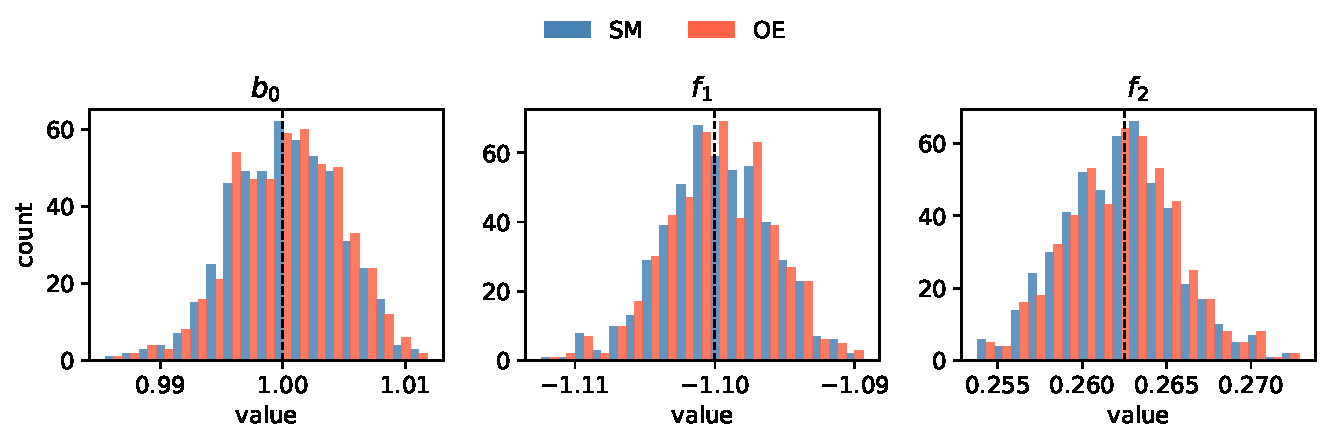
\includegraphics[width=\columnwidth]{experiments/robustness_noisy_data_parameters.pdf}
  \caption{Monte Carlo histograms of the OE-structure parameter estimates
           for SM and OE.
           Dashed vertical lines mark true values.}
  \Description{Three side-by-side histograms of the
    OE-structure parameter estimates (b0, f1, f2) comparing SM
    and OE distributions, with dashed vertical lines at the true
    parameter values.}
  \label{fig:robustness-params}
\end{figure}

\subsection{Effect of Filtered Continuation}
\label{subsec:filtered-continuation}

The second experiment tests whether the filtered continuation strategy
improves the convergence of the OE estimator when the PEM criterion
has multiple local minima.
It exercises the filtered-estimator interface in the same way a user would use
it: the standard and filtered routines return the same model representation and
are evaluated by the same simulation-error computation.
The true system is a third-order OE plant with
\(B(q^{-1})=1\), \(n_k=1\), and
\(F(q^{-1}) = 1 - 2.4q^{-1} + 1.91q^{-2} - 0.504q^{-3}\),
corresponding to poles at $0.9$, $0.8$, and $0.7$.
The input is the three-sine signal
\(u(t) = \sin(2\pi t/18) + \sin(2\pi t/28) + \sin(2\pi t/61)\)
of length $N=1000$, and
white Gaussian noise with $\sigma_v = 30$ is added to the output,
yielding a signal-to-noise ratio of approximately $-6$\,dB.
A Monte Carlo of $M=100$ independent realizations is performed from a
fixed pseudo-random seed;
both estimators use ARX-based initializations and the same
optimization core
(Section~\ref{subsec:nonlinear-optimization-core}):
the standard OE PEM routine proceeds directly to the unfiltered
criterion, whereas the filtered variant first follows the filtered
continuation path before its final unfiltered stage.

Quality is measured by the relative simulation error
$\|y_0 - \hat{y}_s\|_2 / \|y_0\|_2$ on the noise-free output,
and a run is considered successful if this error is below~$5\%$,
a typical practical tolerance for model-based control applications.
Table~\ref{tab:filtered-results} reports the mean and standard deviation
of the error for both routines, as well as the success rate.
The standard OE estimator succeeds in $60\%$ of the Monte Carlo runs
(95\% Wilson confidence interval $[50\%,69\%]$),
with a mean error of $5.7 \times 10^{-2}$.
The filtered variant succeeds in $100\%$ of the runs
(95\% Wilson confidence interval $[96\%,100\%]$) and reduces the
mean error to $2.2 \times 10^{-2}$.
Figure~\ref{fig:filtered-errors} shows the error distribution and a
boxplot of both estimators.
The tenfold increase in computational cost due to the nine filtered
stages is the price paid for achieving a $100\%$ empirical success
rate in this problem.  The experiment is limited to OE because the
cost-function-shaping theory motivating the filtered implementation was
developed for output-error models; the same software pattern is provided for
ARMAX and Box--Jenkins through the filtered routines listed in
Table~\ref{tab:public-api}.

\begin{table}[t]
  \caption{Relative simulation error of OE and OE filtered
           on a non-convex OE-structure PEM problem ($M=100$).}
  \label{tab:filtered-results}
  \centering
  \footnotesize
  \begin{tabular}{lccc}
    \toprule
    Estimator & Mean error & Std error & Success rate ($<5\%$) \\
    \midrule
    OE & $5.69 \times 10^{-2}$ & $4.37 \times 10^{-2}$ & $60\%$ \\
    OE filtered & $2.17 \times 10^{-2}$ & $7.94 \times 10^{-3}$ & $100\%$ \\
    \bottomrule
  \end{tabular}
\end{table}

\begin{figure}[t]
  \centering
  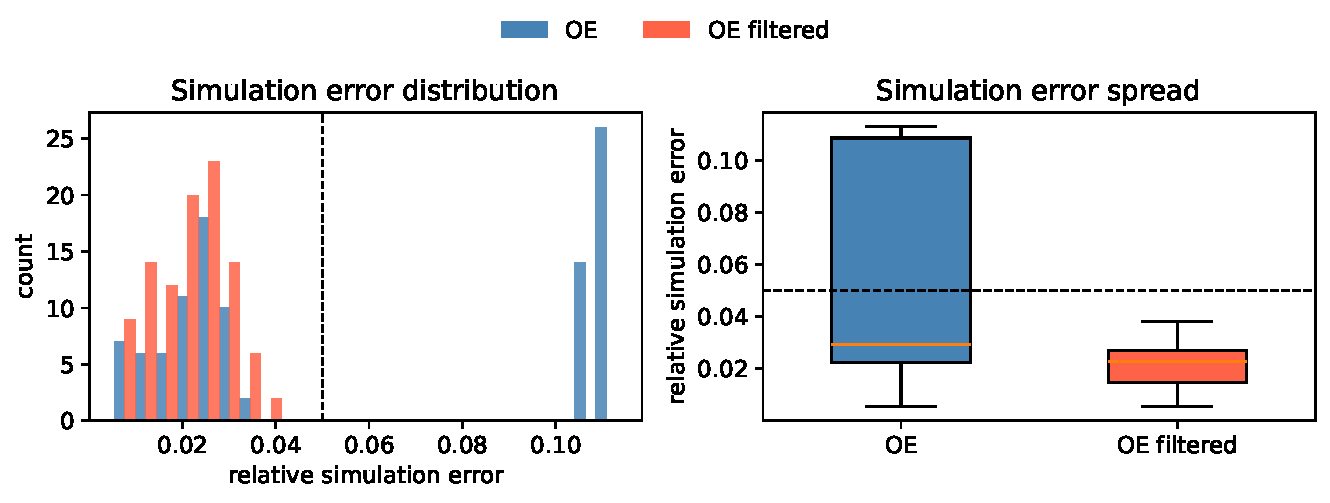
\includegraphics[width=\columnwidth]{experiments/filtered_continuation_oe_errors.pdf}
  \caption{Distribution of the relative simulation error for OE and
           OE filtered on the non-convex problem.
           Dashed line marks the $5\%$ success threshold.}
  \Description{Two panels showing the relative simulation error
    for OE and OE filtered: a histogram comparing their
    distributions, and a boxplot comparing their spreads, with
    a dashed line at the 5 percent success threshold.}
  \label{fig:filtered-errors}
\end{figure}

\section{Conclusion}
\label{sec:conclusion}

\texttt{pysib} is an open-source Python package for parameter
identification of discrete-time SISO systems using classical
polynomial input--output model structures.
It provides a unified interface to estimators for ARX, output-error, ARMAX,
and Box--Jenkins structures, including least-squares, Steiglitz--McBride,
instrumental-variable, correlation, PEM, and filtered PEM routines.  All
estimation routines return the same kind of object: a free-parameter vector
and a five-polynomial dictionary.  This common convention lets users compare
routines and evaluate models through shared prediction and simulation
routines.

The package makes three main contributions.
First, it fills a gap in the open Python ecosystem by delivering a focused,
well-tested implementation of classical polynomial estimators with a compact
API and a consistent model representation that lets users switch between
model structures without changing the downstream evaluation code.
Second, the PEM estimators for non-convex criteria use a specialized
optimization core that combines analytic sensitivity recursions with a
deliberately conservative many-step search; the core is implemented as
compiled C extensions with LAPACK calls, orchestrated from Python.
Third, the toolbox provides open implementations of filtered
continuation methods~\cite{eckhard2013input,eckhard2017cost} for non-convex
PEM criteria; these methods progressively relax data filters
to drive the estimate toward the original PEM criterion.

Numerical experiments show that under noisy data the SM and OE
estimates are centered close to the true parameters, and that the
filtered continuation strategy raises the success rate on a
non-convex OE-structure PEM problem from $60\%$ to $100\%$ of the runs.
The complete source code, unit tests, user manual, and reproducible drivers
are included in the accompanying CALGO software artifact.

\begin{acks}
This work was supported by CNPq/Brazil.
\end{acks}

\bibliographystyle{ACM-Reference-Format}
\bibliography{references}

\end{document}
